\documentclass[border=10pt]{standalone}
\usepackage{pgfplots}
\pgfplotsset{compat=1.18}

\begin{document}
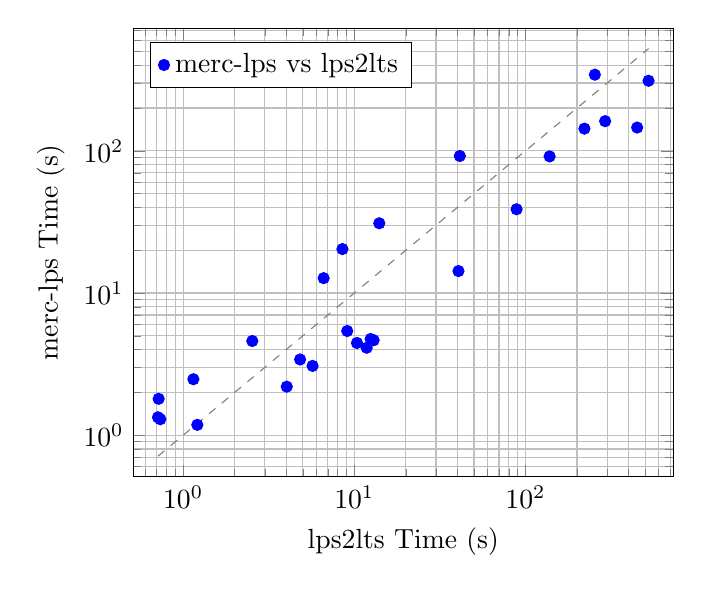
\begin{tikzpicture}
\begin{axis}[
  xlabel={lps2lts Time (s)},
  ylabel={merc-lps Time (s)},
  grid=both,
  legend pos=north west,
  enlargelimits=0.05,
  xmode=log,
  ymode=log
]
\addplot[only marks, mark=*, color=blue] coordinates {
  (9.08581, 5.40485)
  (88.6944, 38.8278)
  (4.02824, 2.19461)
  (449.174, 145.745)
  (10.3596, 4.45519)
  (1.20961, 1.18291)
  (12.9618, 4.6538)
  (12.4506, 4.74976)
  (5.70213, 3.07147)
  (40.5874, 14.2692)
  (11.8073, 4.12168)
  (220.945, 143.179)
  (254.192, 343.211)
  (4.82159, 3.40902)
  (138.329, 91.3591)
  (523.479, 310.84)
  (0.71234, 1.33678)
  (0.735109, 1.29578)
  (2.5338, 4.59683)
  (6.61761, 12.7199)
  (1.1472, 2.47511)
  (13.9852, 30.9389)
  (8.52066, 20.3725)
  (291.973, 161.64)
  (0.718847, 1.80215)
  (41.3398, 91.9614)
};
\addlegendentry{merc-lps vs lps2lts}
\addplot[no marks, dashed, gray, forget plot] coordinates {(0.71234, 0.71234) (523.479, 523.479)};
\end{axis}
\end{tikzpicture}
\end{document}
